\section{Diskussion}
\label{sec:Diskussion}
Die Evakuierungskurven der Pumpen (vgl. Abb. \ref{fig:drehEvac} und \ref{fig:turboEvac}) sind erwartungsgemäß aufgenommen worden.
Bei der Drehschieberpumpe ist eine Einteilung in 3 Bereiche möglich.
Lediglich waren bei der Turbomolekularpumpe die Messintervalle zu groß und die Bereiche des konstanten logarithmischen Ausdruckes sind nicht einwandfrei erkennbar.
Durch eine momentane Verkürzung der Messintervalle innerhalb der ersten \qty{30}{\second} könnte eine deutlich bessere Gliederung der einzelnen Abschnitte gelingen.
Demnach profitiere auch die Genauigkeit der damit berechneten Saugvermögen.

Bei allen Leckratenmessungen konnte für beide Pumpentypen ein linearer Druckanstieg gemessen werden 
(vgl. Abb. \ref{fig:drehLeck05} bis \ref{fig:drehLeck100} und \ref{fig:turboLeck2} bis \ref{fig:turboLeck5}).

\begin{figure}
    \centering
    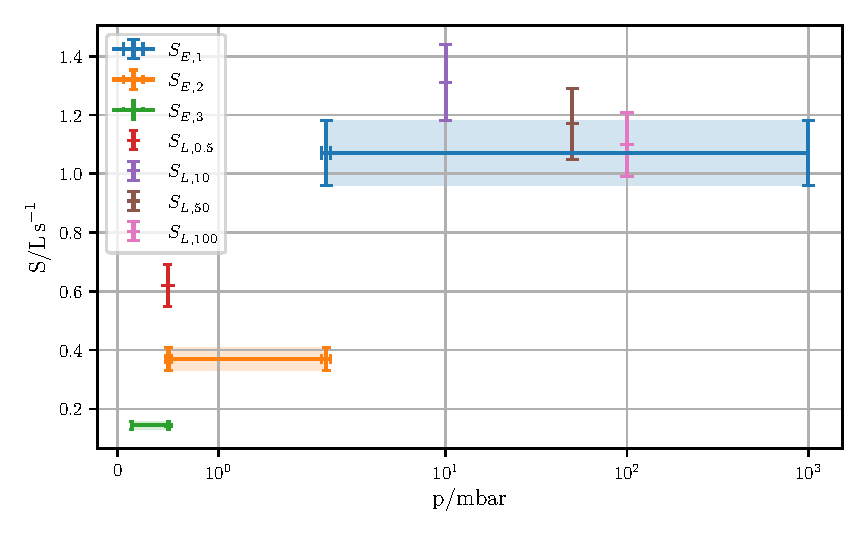
\includegraphics[width=0.8\textwidth]{abb/plot1.pdf}
    \caption{Die Saugvermögen der verschiedenen Messreihen und Messmethoden zur Drehschieberpumpe im Vergleich.}
    \label{fig:dreh}
\end{figure}
\begin{figure}
    \centering
    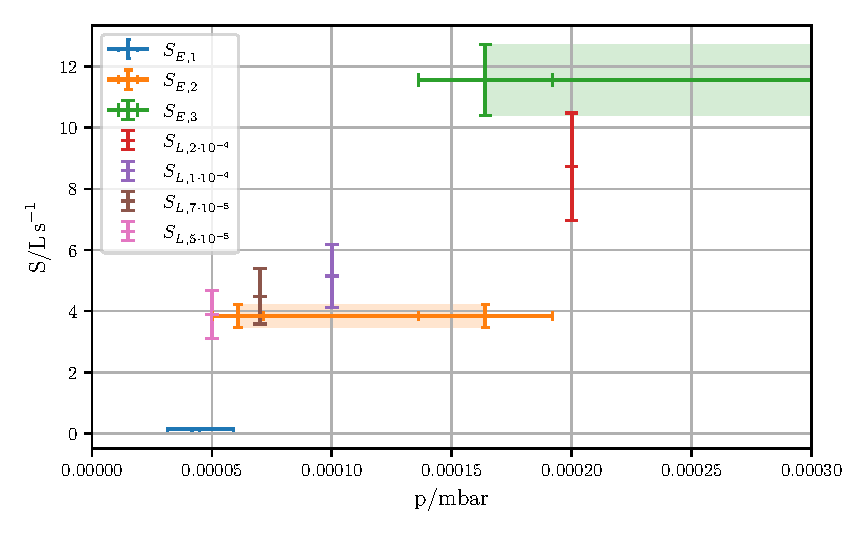
\includegraphics[width=0.8\textwidth]{abb/plot2.pdf}
    \caption{Die Saugvermögen der verschiedenen Messreihen und Messmethoden zur Turbomolekularpumpe im Vergleich.}
    \label{fig:turbo}
\end{figure}
In \autoref{fig:dreh} sind die verschiedenen Saugvermögen der einzelnen Methoden und Messreihen der Drehschieberpumpe aufgeführt.
In \autoref{fig:turbo} die der Turbomolekularpumpe. Bei der Drehschieberpumpe bietet sich aufgrund der großen Unterschiede der Druckbereiche
ein halblogarithmischer Plot an.
Alle Saugvermögen sind samt ihrer fortgepflanzten Fehlerbalken dargestellt.
Da aus den Berechnungen der Evakuierungskurven ein Saugvermögen für einen Druckbereich resultiert,
ist der Fehlerwert über den gesamten Druckbereich als farbig hinterlegter Balken dargestellt.
Im Idealfall liegen die Saugvermögen aus der Leckratenmessung, abhängig von ihrem Startdruck, innerhalb dieser Fehlerbalken um eine Äquivalenz der beiden Methoden zu zeigen.
Ferner ist ein Überschneiden der Fehler ausreichend um eine Übereinstimmung nicht ausschließen zu können.
Dies ist der Fall beim dritten Abschnitt der Drehschieberpumpe sowie beim zweiten und dritten Abschnitt der Turbomolekularpumpe.


\begin{table}
    \centering
    \caption{Die Saugvermögen der verschiedenen Messreihen und Messmethoden im Vergleich.}
    \label{tab:disk}
    \begin{tabular}{c|S[table-format=1.3(3)]c|S[table-format=2.2(2)]S[table-format=2.1]}
        \toprule
        Pumpe: &\multicolumn{2}{c}{Drehschieber}&\multicolumn{2}{c}{Turbomolekular}\\
        \midrule
        Saugvermögen & {$S/\unit{\litre\per\second}$} & $\Delta S/\unit{\percent}$ & {$S/\unit{\litre\per\second}$} & {$\Delta S/\unit{\percent}$} \\
        \midrule
        $S_{E,1}$ & 1.07(11) & 16.4 - 30.1 & 11.56(1.16) & 85.0 \\
        $S_{E,2}$ & 0.37(4) & 71.1 - 75.8 & 3.84(38) & 95.0 \\
        $S_{E,3}$ & 0.144(14) & 88.8 - 90.6 & 0.14(1) & 99.8 \\
        $S_{L,1}$ & 0.62(7) & 51.6 - 59.5 & 8.72(1.76) & 88.7 \\
        $S_{L,2}$ & 1.31(13) & 2.3 - 14.4 & 5.15(1.04) & 93.3 \\
        $S_{L,3}$ & 1.17(12) & 8.6 - 23.5 & 4.48(90) & 94.2 \\
        $S_{L,4}$ & 1.10(11) & 14.1 - 28.1 & 3.89(78) & 94.5 \\
        \bottomrule
    \end{tabular}
\end{table}
Die Herstellerangaben der Pumpen sind $\qty{77}{\liter\per\second}$ für die Turbomolekularpumpe und $1.28$ bis $1.53 \unit{\liter\per\second}$ für die Drehschieberpumpe.
Zumindest kann der Wert $S_{L,2}$, mit $p_g=\qty{10}{\milli\bar}$ der Drehschieberpumpe den Hersteller in seinem Fehler bestätigen.
Die Ergebnisse sind samt ihrer relativen Abweichungen nach
\begin{equation}
    \Delta S = \left|\frac{S_{lit}-S_{exp}}{S_{lit}}\right|
\end{equation}
in \autoref{tab:disk} aufgeführt.
Es muss berücksichtigt werden, dass lediglich das effektive Saugvermögen
\begin{equation*}
    S_{eff} = \frac{S_0\cdot L}{S_0 + L}
\end{equation*}
mit dem Leitwert $L$ der Rohre und dem theoretischen Saugvermögen $S_0$ bestimmt werden kann.

Der Hersteller ist unter professionellen Laborbedingungen daran interessiert mit einer höchstmöglichen Saugleistung sein Produkt zu bewerben.
Demnachzufolge ist jede mögliche Erhöhung des Strömungswiderstandes zu minimieren, beispielsweise durch ein regelmäßiges Ausheizen der Messapparatur und der Vakuumpumpe.
Zudem sollte in Anbetracht der benötigten Desorptionsenegie während einer möglichst tiefen Temperatur gemessen werden, damit die Energieschwelle der Adsorbierten und durch Diffusion
durchdringenden Teilchen möglichst groß ist. Abzuwägen ist demnach jedoch, ob und wie eine tiefere Temperatur andere kontraproduktive Einflüsse ausübt.
\newpage

\begin{figure}
    \centering
    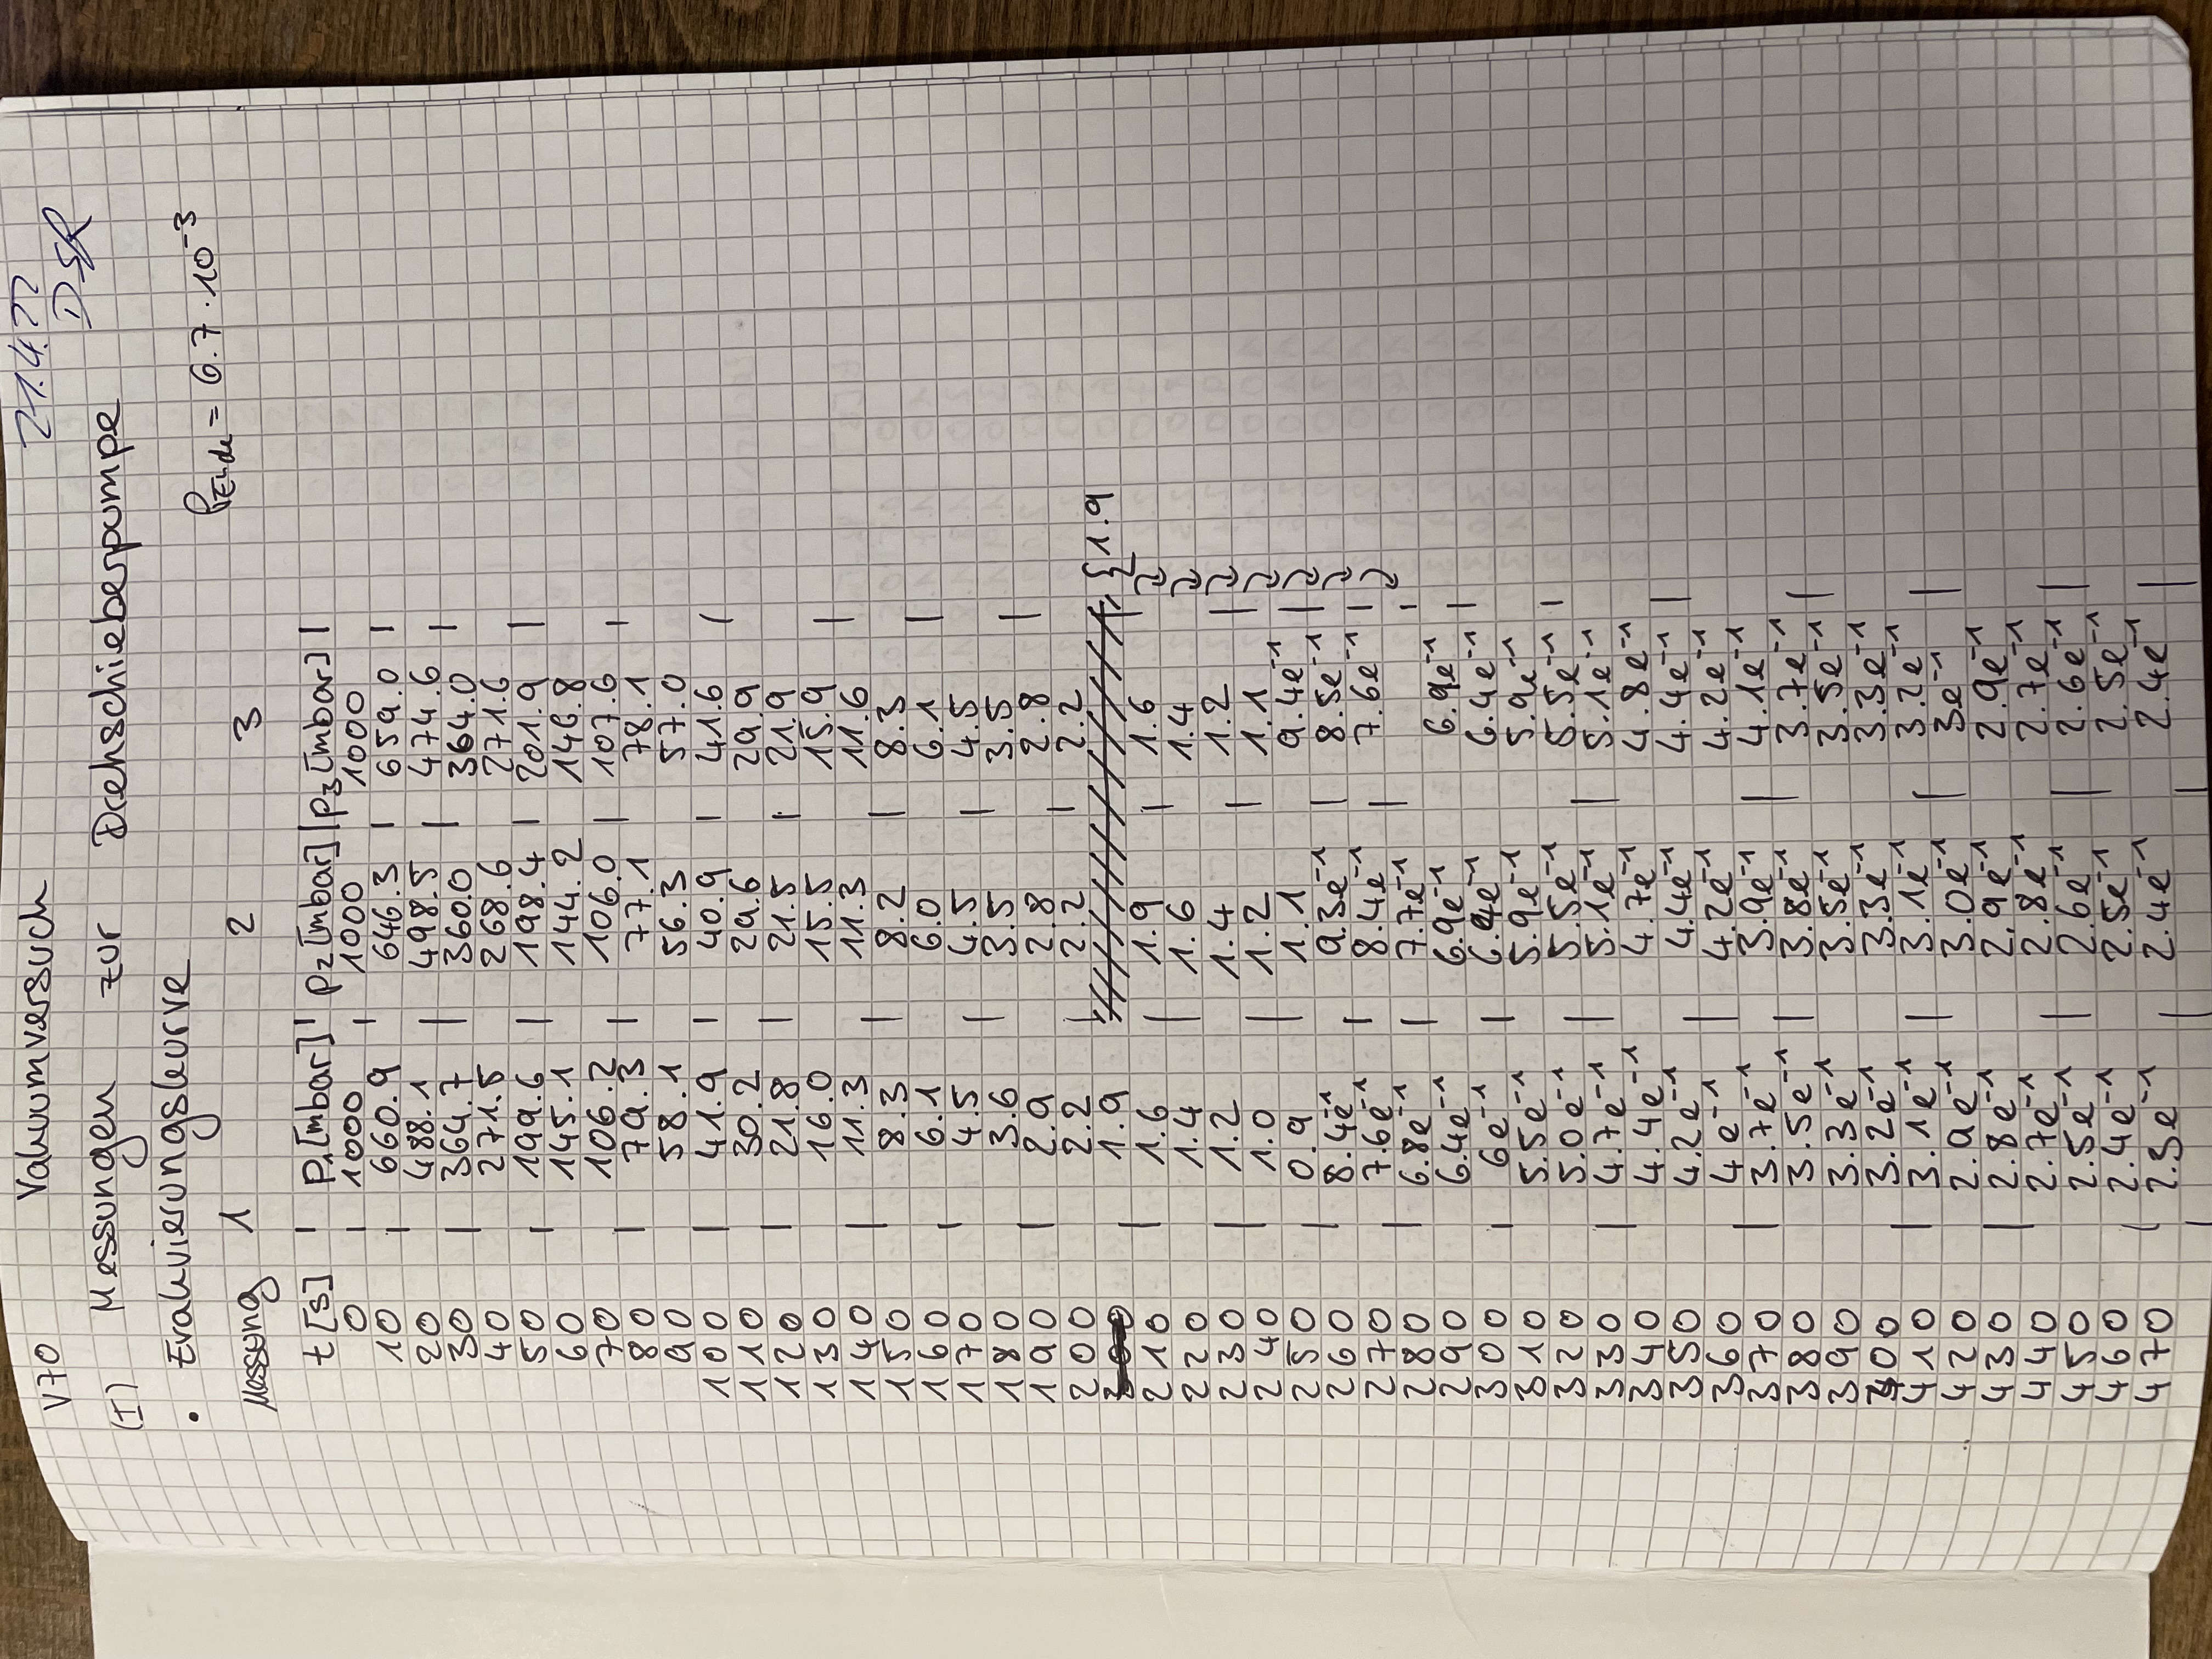
\includegraphics[width=0.7\textwidth]{abb/IMG_3226.jpg}
\end{figure}
\begin{figure}
    \centering
    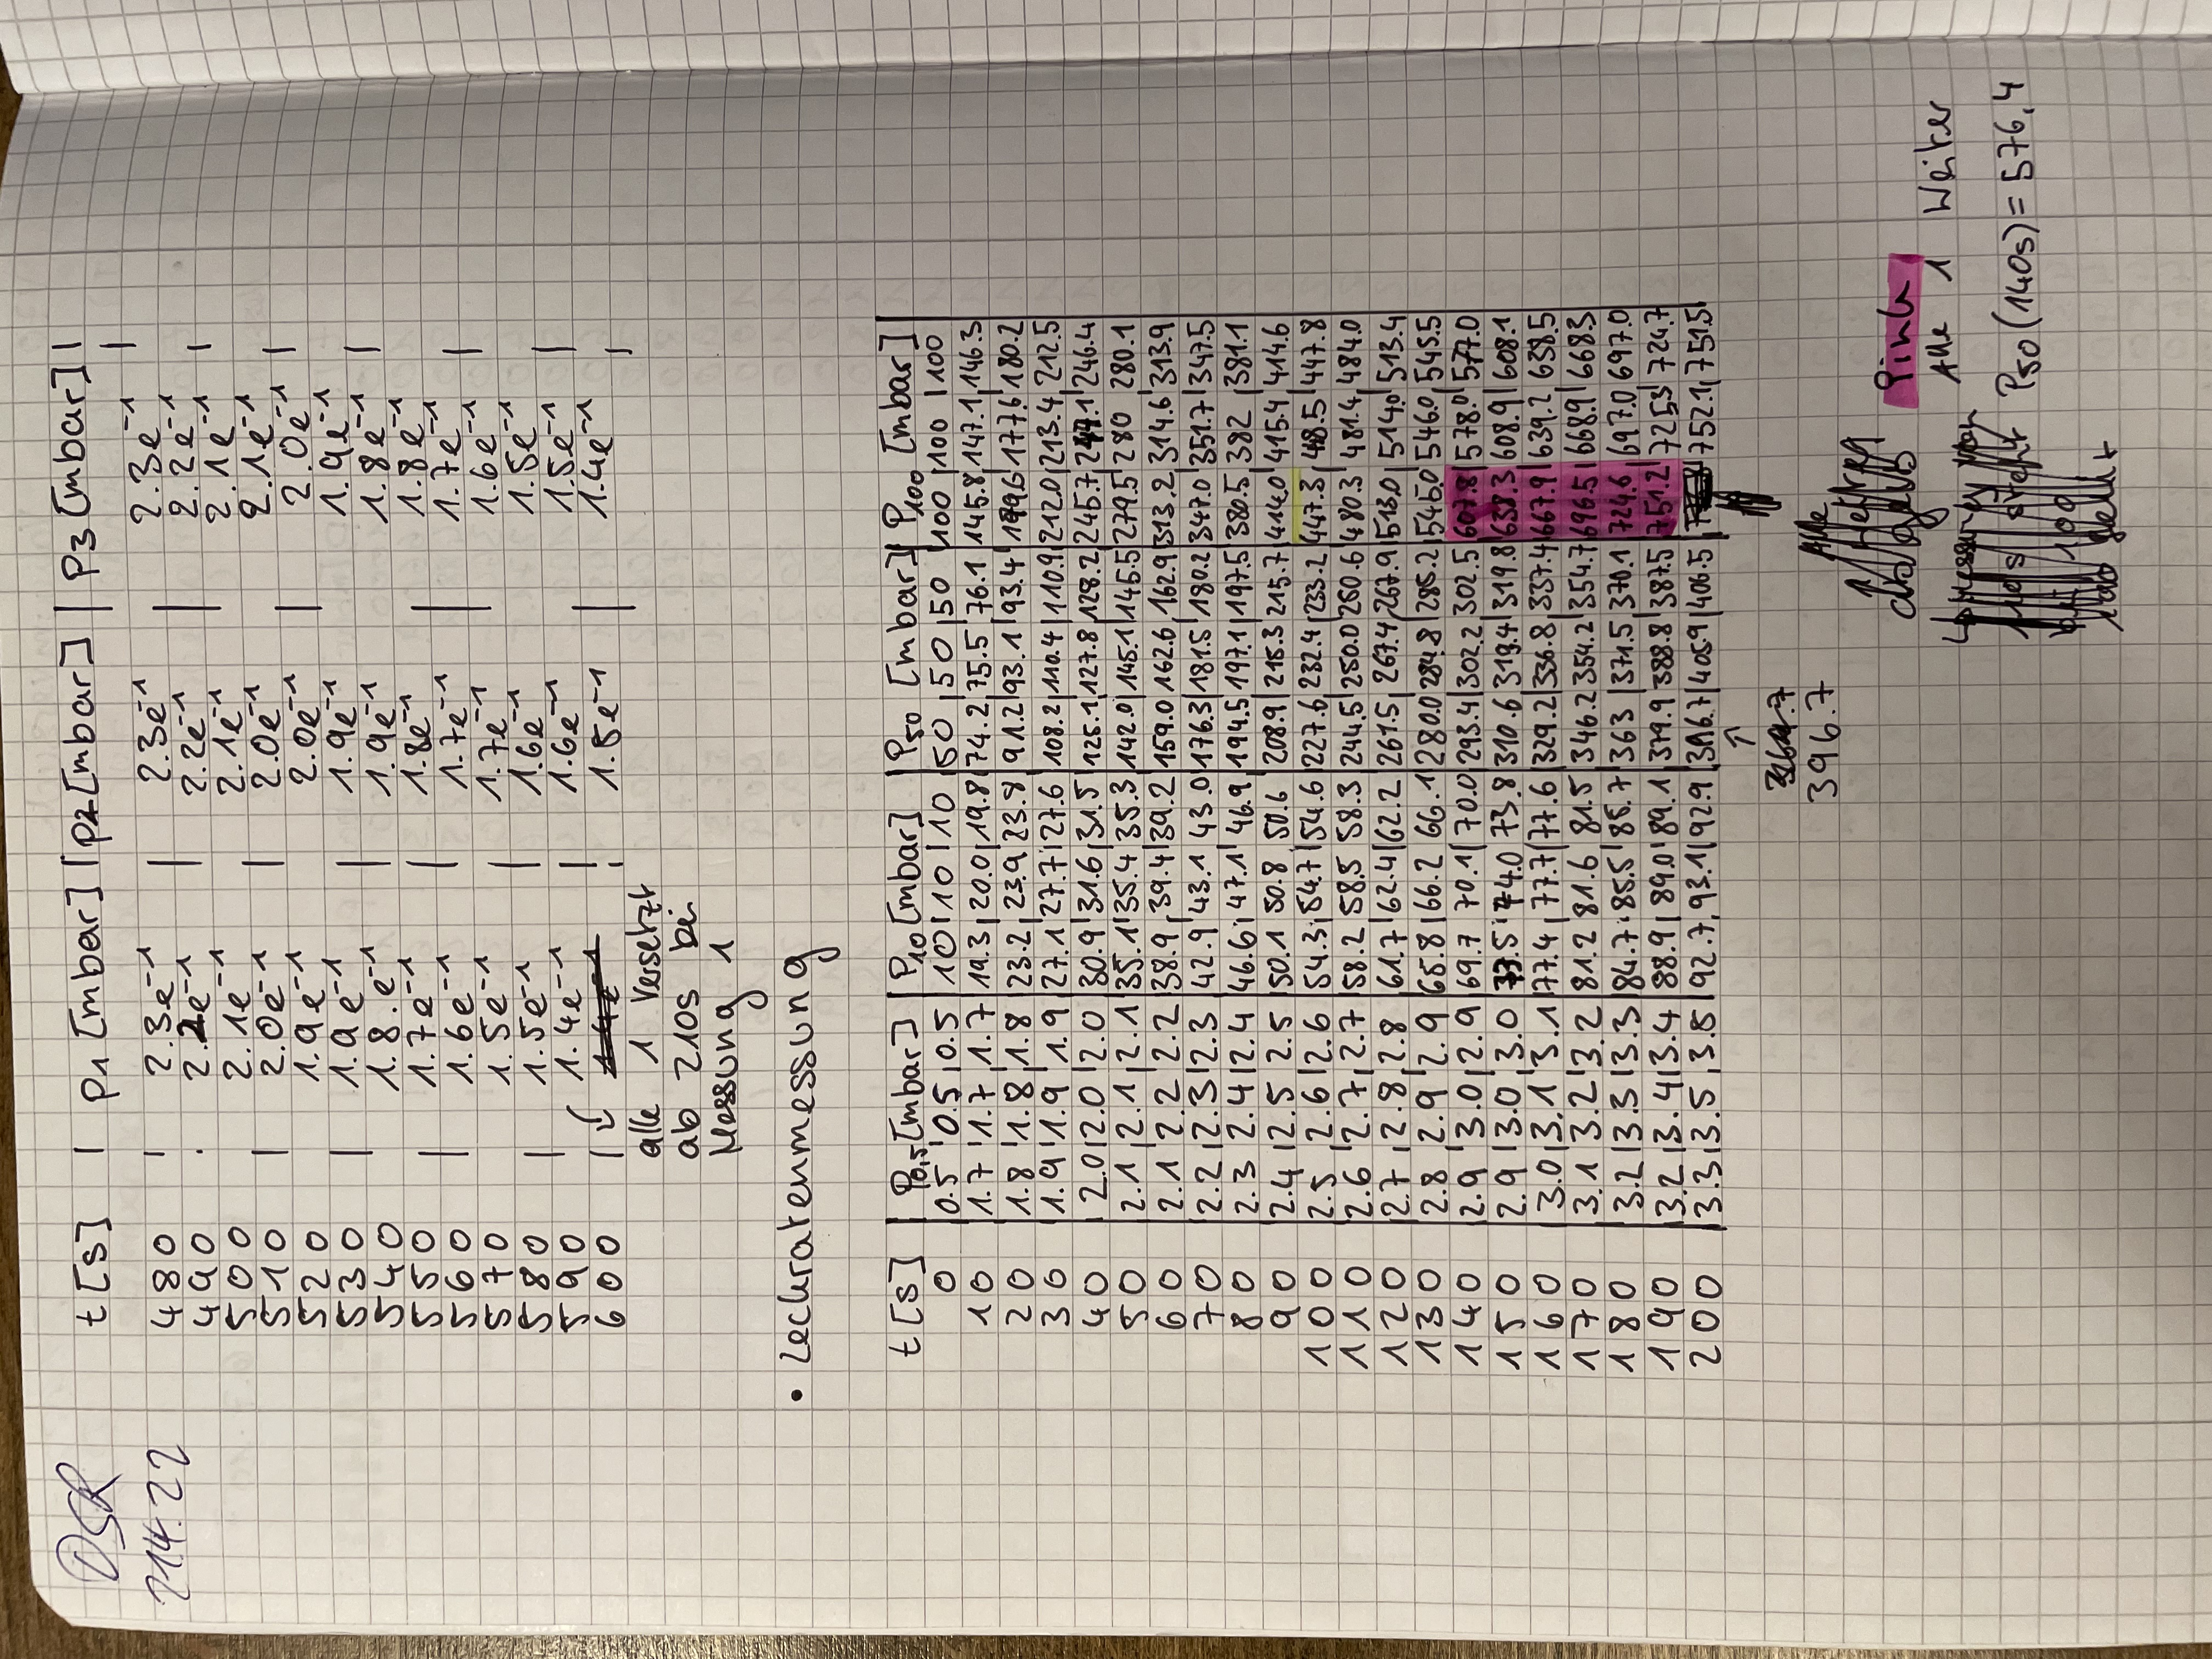
\includegraphics[width=0.7\textwidth]{abb/IMG_3227.jpg}
\end{figure}
\begin{figure}
    \centering
    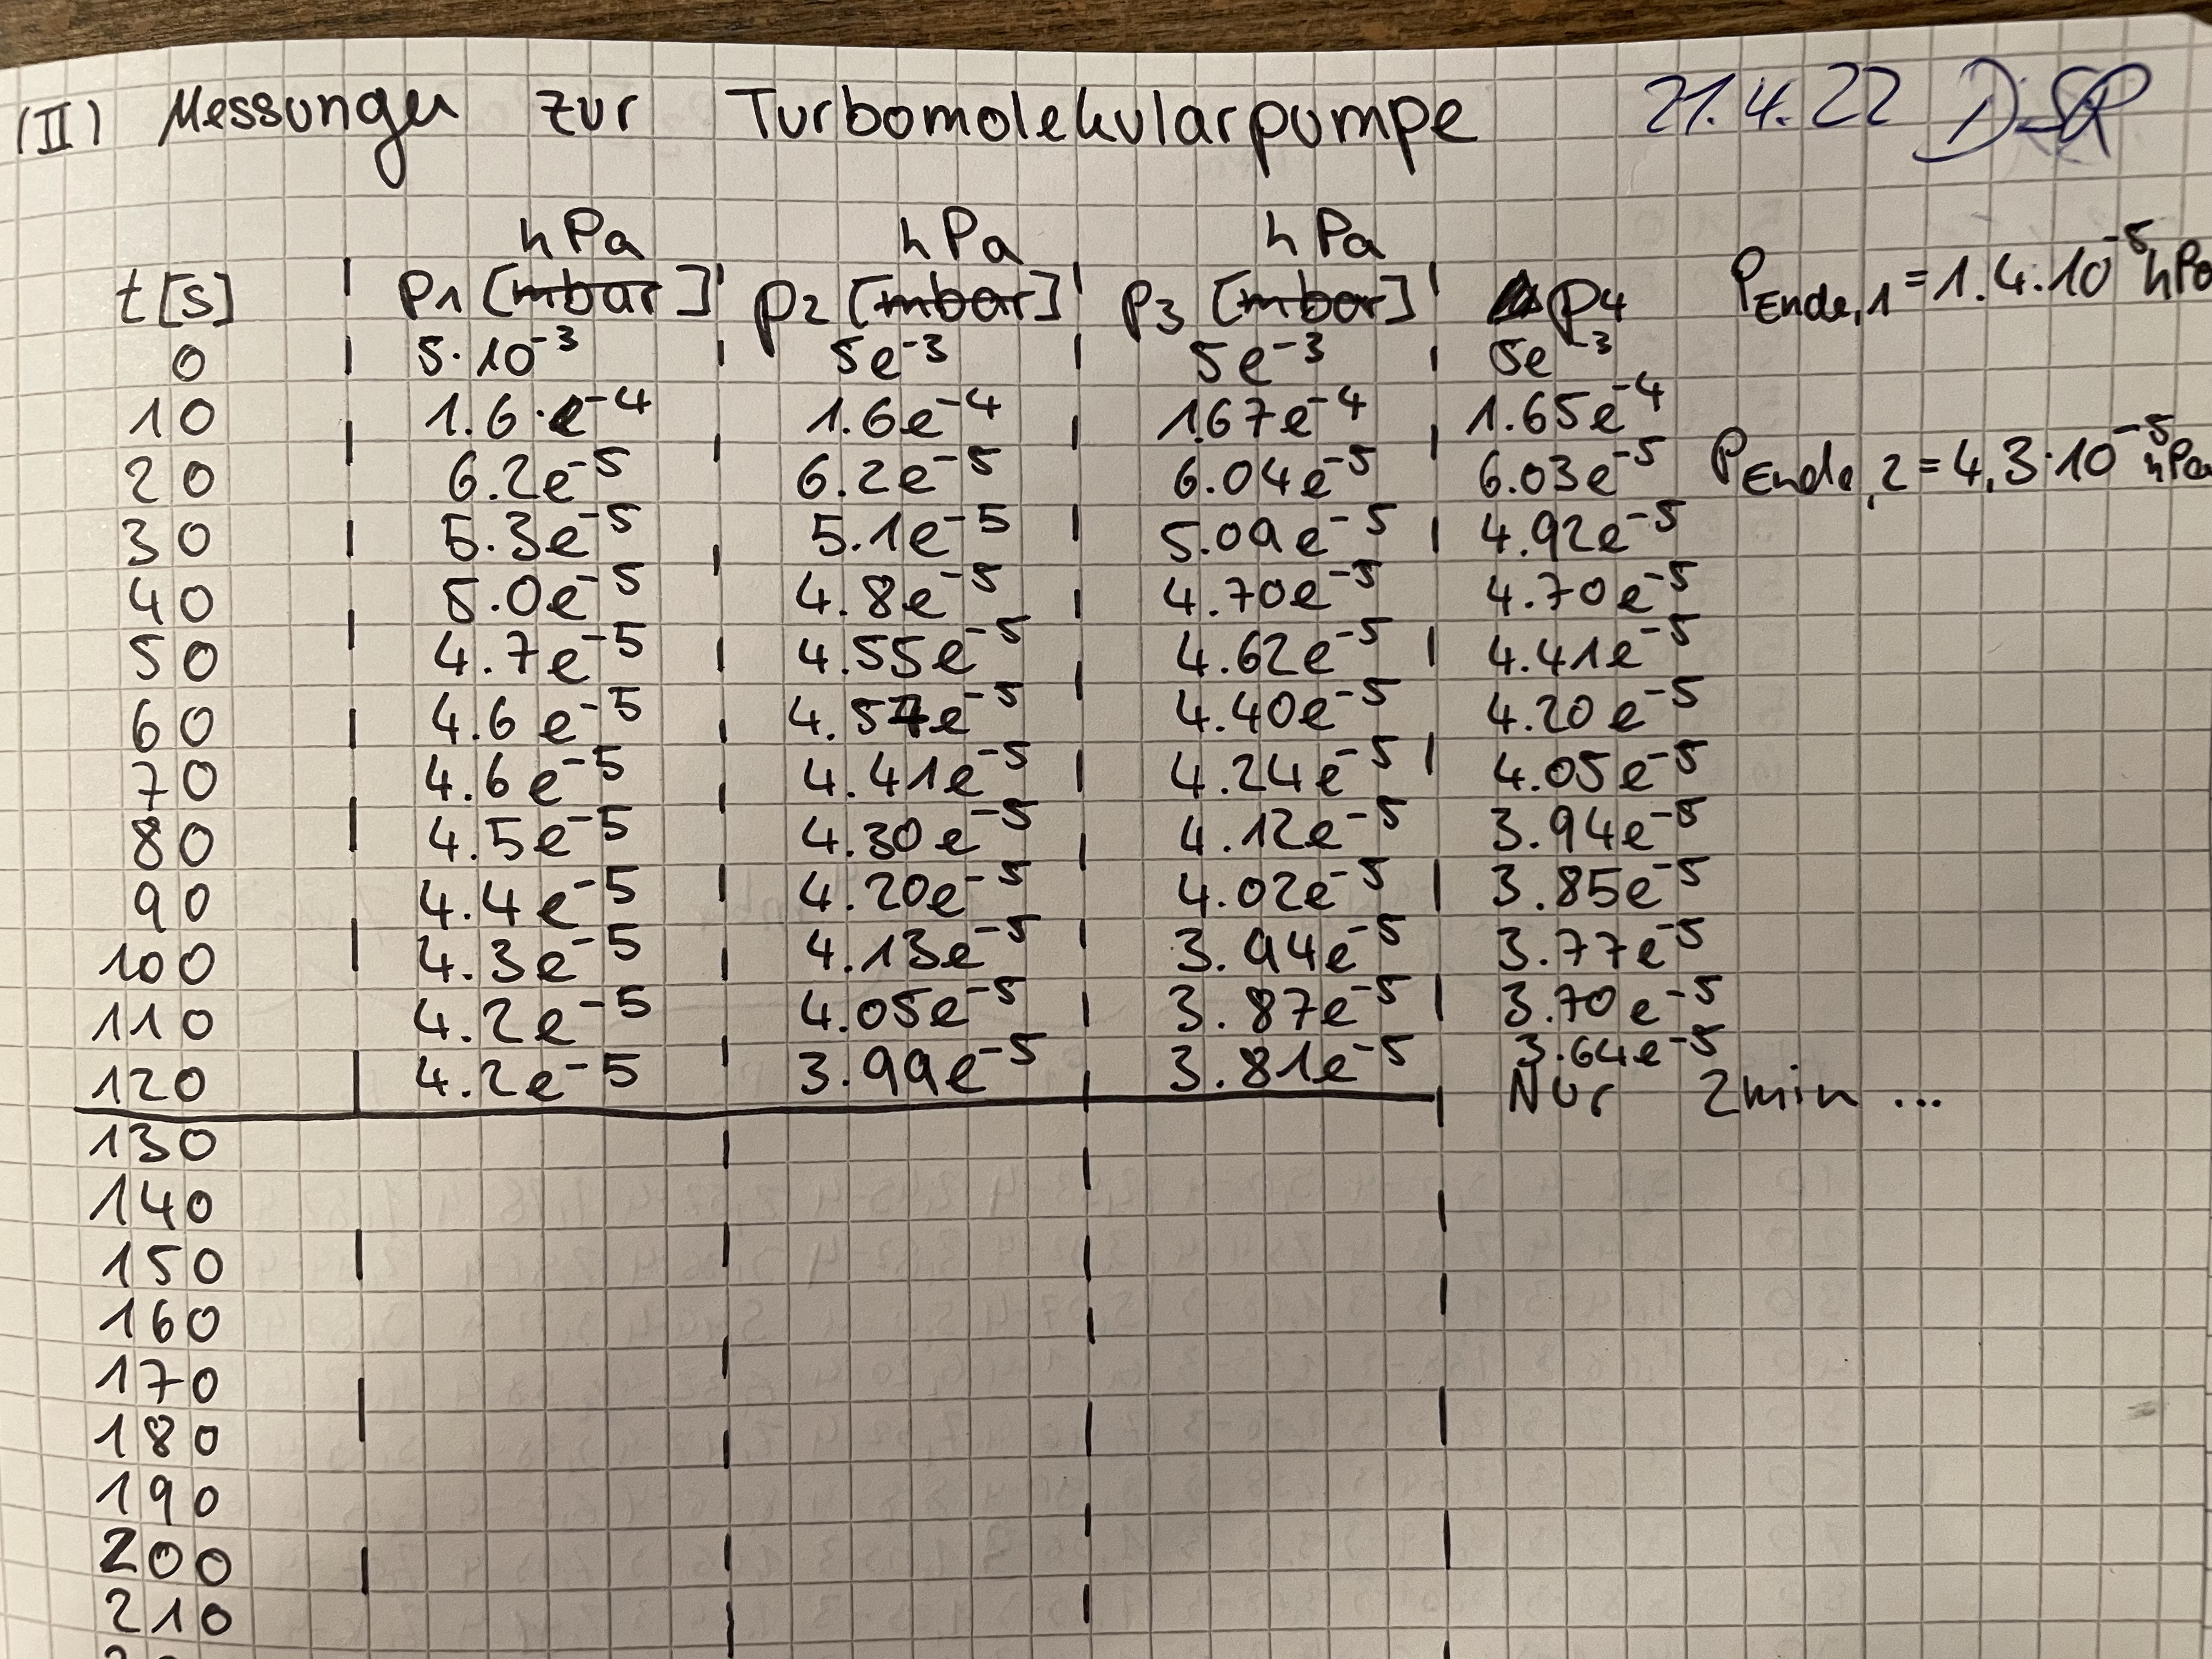
\includegraphics[width=0.7\textwidth]{abb/IMG_3228.jpg}
\end{figure}
\begin{figure}
    \centering
    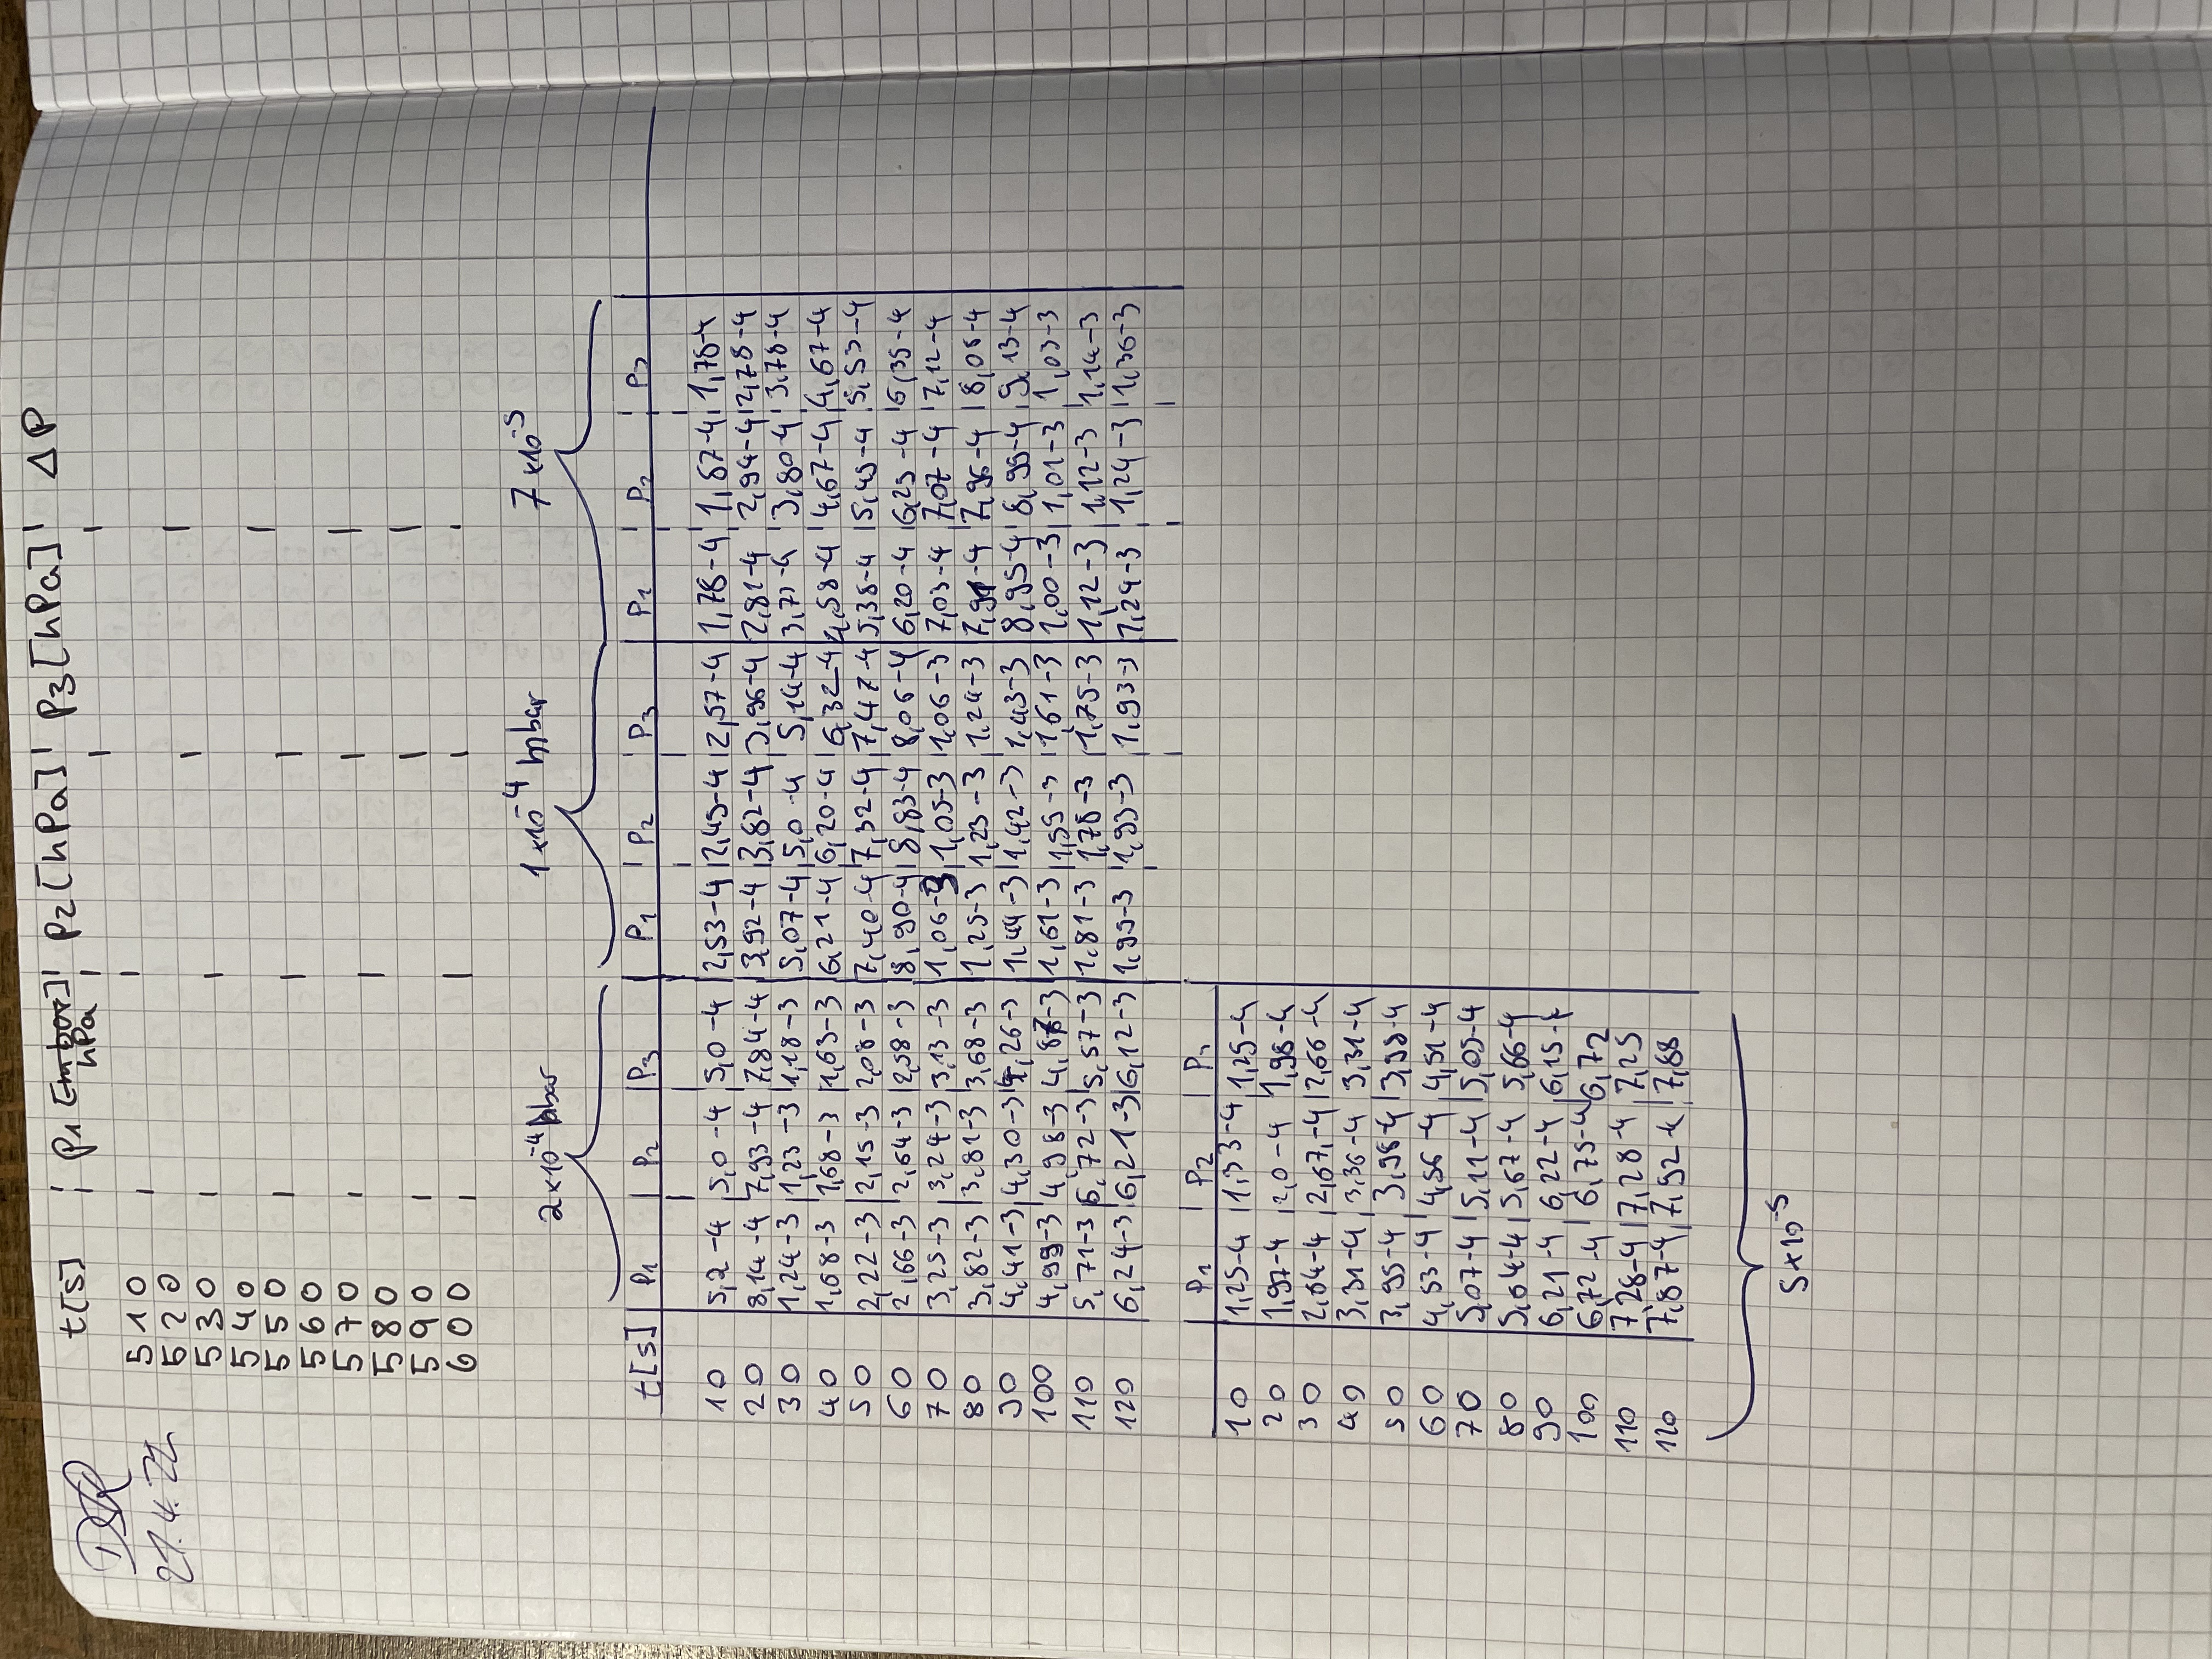
\includegraphics[width=0.7\textwidth]{abb/IMG_3229.jpg}
\end{figure}